%%%%%%%%%%%%%%%%%%%%%%%%%%%%%%%%%%%%%%%%%%%%%%%%%%%%%%%%%%%%%%%%%%%%%%%%%%
%%
%%	Author Submission Template for Operations Research (OPRE)
%%	INFORMS, <informs@informs.org>
%%	Ver. 1.00, June 2024
%%  Modified by Jiheng Zhang @ UST
%%
%%%%%%%%%%%%%%%%%%%%%%%%%%%%%%%%%%%%%%%%%%%%%%%%%%%%%%%%%%%%%%%%%%%%%%%%%%
%
% Use dblanonrev for Double Anonymous Review submission
% Use sglanonrev for Single Anonymous Review submission
% For example, submission to INFORMS Mathematics of Operation Research, MOOR will have
% \documentclass[moor,dblanonrev]{style/informs4}
%
% \documentclass[opre,dblanonrev]{style/informs4}
\documentclass[opre,sglanonrev]{style/informs4}
% \usepackage{eqndefns-left} % For checking the display equation width and equation environment definitions %

\bibliographystyle{style/informs2014}
\usepackage{natbib}
 \bibpunct[, ]{(}{)}{,}{a}{}{,}%
 \def\bibfont{\small}%
 \def\bibsep{\smallskipamount}%
 \def\bibhang{24pt}%
 \def\newblock{\ }%
 \def\BIBand{and}%

\usepackage{hyperref}       % hyperlinks
\hypersetup{
  colorlinks=true,
  linkcolor=red,
  urlcolor=magenta,
  citecolor=blue
}
\usepackage{bookmark}       % improved PDF bookmarks (loads after hyperref)

% Note: amsmath, amssymb, amsfonts, graphicx, color, url already loaded by informs4.cls
\usepackage{subfiles}
\usepackage{booktabs}
\usepackage{mathtools}
\usepackage{microtype}
\usepackage[english]{babel}

\usepackage{pgfplots}
\usepgfplotslibrary{groupplots,dateplot}

\usepackage{pgfplotstable}

\usepackage{tikz}
\usetikzlibrary{patterns,shapes.arrows,arrows,shapes}
\usetikzlibrary{arrows.meta, calc, topaths, positioning, automata}
\pgfplotsset{compat=newest}
\pgfplotsset{compat=1.17}

\tikzset{
	cir/.style ={
	ellipse, %矩形节点
	minimum width =15pt, %最小宽度
	minimum height =23pt, %最小高度
	align=center,
	text width=20pt,
	inner sep=2pt, %文字和边框的距离
	draw=black, %边框颜色}
	% font=\tiny	
	}
}

\tikzset{
	pcir/.style ={
	circle, %矩形节点
	minimum width =15pt, %最小宽度
	minimum height =15pt, %最小高度
	align=center,
	text width=20pt,
	inner sep=2pt, %文字和边框的距离
	draw=blue, %边框颜色}
	% font=\tiny
	}
}

\tikzset{
box/.style ={
rectangle, %矩形节点
rounded corners =3pt, %圆角
minimum width =25pt, %最小宽度
minimum height =20pt, %最小高度
inner sep=2pt, %文字和边框的距离
draw=black %边框颜色}
}
}

% Load the fix-cm package
\usepackage{fix-cm}
% Manually declare missing font shapes if necessary
\DeclareFontShape{OML}{cmm}{b}{it}{<->cmmib10}{}
\DeclareFontShape{OMS}{cmsy}{b}{n}{<->cmsy10}{}

%\OneAndAHalfSpacedXI
\OneAndAHalfSpacedXII % Current default line spacing
%%\DoubleSpacedXI
%%\DoubleSpacedXII

%% Setup of the equation numbering system. Outcomment only one.
%% Preferred default is the first option.
\EquationsNumberedThrough    % Default: (1), (2), ...
%\EquationsNumberedBySection % (1.1), (1.2), ...

%% Setup of theorem styles. Outcomment only one.
%% Preferred default is the first option.
\TheoremsNumberedThrough     % Preferred (Theorem 1, Lemma 1, Theorem 2)
%\TheoremsNumberedByChapter  % (Theorem 1.1, Lema 1.1, Theorem 1.2)
\ECRepeatTheorems  %  

% For new submissions, leave this number blank.
% For revisions, input the manuscript number assigned by the on-line
% system along with a suffix ".Rx" where x is the revision number.
% \MANUSCRIPTNO{MOOR-0001-2024.00}

%%%%%%%%%%%%%%%%
\begin{document}
%%%%%%%%%%%%%%%%

% Outcomment only when entries are known. Otherwise leave as is and
%   default values will be used.
%\setcounter{page}{1}
%\VOLUME{00}%
%\NO{0}%
%\MONTH{Xxxxx}% (month or a similar seasonal id)
%\YEAR{0000}% e.g., 2005
%\FIRSTPAGE{000}%
%\LASTPAGE{000}%
%\SHORTYEAR{00}% shortened year (two-digit)
%\ISSUE{0000} %
%\LONGFIRSTPAGE{0001} %
%\DOI{10.1287/xxxx.0000.0000}%

% Author's names for the running heads
% Sample depending on the number of authors;
% \RUNAUTHOR{Jones}
% \RUNAUTHOR{Jones and Wilson}
% \RUNAUTHOR{Jones, Miller, and Wilson}
% \RUNAUTHOR{Jones et al.} % for four or more authors
% Enter authors following the given pattern:
%\RUNAUTHOR{}

% Title or shortened title suitable for running heads. Sample:
% \RUNTITLE{}

% Enter the full title:
\TITLE{An important and impactful paper}

\ARTICLEAUTHORS{%
%\AUTHOR{John Doe,\textsuperscript{a} Jane Smith,\textsuperscript{b}}
%\AFF{\textsuperscript{a}Department of Industrial Engineering, University of XYZ, \EMAIL{john.doe@xyz.edu; \textsuperscript{b}Department of Computer Science, University of ABC, \EMAIL{jane.smith@abc.edu}} 
% Enter all authors
}

\ABSTRACT{
    % big background
    Stochastic control in multi-class queueing networks has been extensively studied primarily focusing on minimizing operational costs (e.g., waiting, abandonment). 
    % what is novel
    However, in many real-world applications, the system operator must balance the trade-off between waiting costs and maximizing immediate rewards when assigning customers to service units.
    This necessitates the integration of learning algorithms that focus on maximizing immediate rewards through matching, and stochastic control methods that aim to minimize waiting costs by managing queue dynamics.
    % what is our model
    Specifically, we consider a multi-class queueing system where each customer type is associated with a waiting cost and a feature vector. Each service unit consist of multiple idential servers each with a fixed service rate and a parameter. The inner product of the customer feature vector and the server parameter determines the reward when a customer is assigned to a server.
    % What we do (challenge, results, methodology)
    When the server parameters are known, we design a priority rule based on fluid approximation and demonstrate its asymptotic optimality, effectively balancing the trade-offs between reward maximization and waiting cost minimization. 
    When the server parameters are unknown, we incorporate an online learning algorithm into the system control, achieving a regret bound of order $O(\ln T)$.
    % Numerical experiments
    Numerical experiments demonstrate the effectiveness of our proposed algorithms in balancing the trade-offs between immediate rewards and waiting costs.
}%

%\FUNDING{This research was supported by [grant number, funding agency].}

\KEYWORDS{Stochastic control, Queueing network,Uncertainty, Online learning, Optimization} 

%\HISTORY{Received: Month DD, YYYY; Accepted: Month DD, YYYY; Published Online: Month DD, YYYY}

\maketitle
%%%%%%%%%%%%%%%%%%%%%%%%%%%%%%%%%%%%%%%%%%%%%%%%%%%%%%%%%%%%%%%%%%%%%%

% Text of your paper here
\section{Introduction}

%Motivation
Queueing control problems are widely studied in stochastic control, with applications in telecommunications, emergency services, project management, and more. In a traditional multi-class queueing control problem, the decision maker must design a priority rule—such as the $c\mu$ rule—to determine which type of customer to serve based on certain exogenous properties of the system. The primary objective is to minimize operational costs, including waiting costs and abandonment.

%Real world 

\cite{Erlang1948,Dantzig1955,Dynkin1956,Bellman1957DP,Little1961,Skorokhod1961,McKean1965,Iglehart1965}

\section{Model}

\begin{tikzpicture}[scale=1.5]
    \label{fig:N-model-rework}
    % Draw axes
    \draw [<->,thick] (0,5) node (yaxis) [above] {$x_2$}
        |- (5,0) node (xaxis) [right] {$x_1$};
    % Draw two intersecting lines
    \draw (0,0) coordinate (a_1) -- (1.6,2) coordinate (a_2);
    \draw (1.6,2) coordinate (b_1) -- (1.6,4.75) coordinate (b_2);
    \draw[dashed] (0,4.88) -- (2.7111,0);
    \node at (3.4,0.4) {$s_2(\bar W(t))=K_2$};

    \coordinate (c) at (intersection of a_1--a_2 and b_1--b_2);
    % Draw lines indicating intersection with y and x axis. Here we use
    % the perpendicular coordinate system
    \draw[dashed] (yaxis |- c) node[left] {$K_2$}
        -| (xaxis -| c) node[below] {$\frac{\mu_2K_2}{\mu_1}$};
    \draw[dashed] (2.2, 0.05) -- (2.2,0) node[below] {$K_1$};
    % Draw a dot to indicate intersection point

    \coordinate (a) at (2.4,0.8);
    \fill[red] (a) circle (1pt);
    \draw[blue] (a) -- (1.6,0.8);

    \coordinate (b) at (1.94,0.9);
    \fill[red] (b) circle (1pt);
    \draw[blue] (b) -- (1.44,1.8);
\end{tikzpicture}

\section{Conclusion}
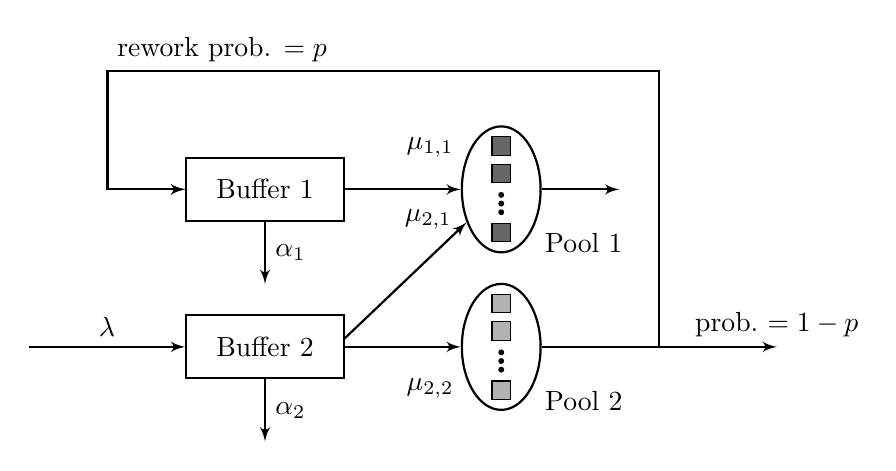
\begin{tikzpicture}[auto, >=latex']
    \everymath{\displaystyle}
    \tikzstyle{every picture}+=[remember picture]

    \tikzstyle{coor-format} = [coordinate]
    \tikzstyle{b-format} = [draw=black, thick,
                            minimum height=0.8cm, minimum width=2cm]
    \tikzstyle{s1-format} = [rectangle, draw=black, fill=black!60]
    \tikzstyle{s2-format} = [rectangle, draw=black, fill=black!30]
    \tikzstyle{p-format} = [ellipse, draw=black, thick,
                            minimum height=1.6cm, minimum width=1cm]

    \node [coor-format] (In1) {};
    \node [b-format, right of=In1, node distance=2cm] (Buf1) {Buffer 1};
    \draw [draw,->, thick] (In1) -- (Buf1);

    \node [coor-format, below of=Buf1, node distance=1.2cm] (Abd1) {};
    \draw [draw,->, thick] (Buf1) -- node {$\alpha_1$} (Abd1);

    \node [p-format, right of=Buf1, node distance=3cm, label=-45:Pool 1,
           label=150:{$\mu_{1,1}$}, label=-165:{$\mu_{2,1}$}] (Pool1) {};
    \draw [draw,->, thick] (Buf1) -- (Pool1);

    \node [coor-format, right of=Pool1, node distance=1.5cm] (Out1) {};
    \draw [draw,->, thick] (Pool1) -- (Out1);

    \node [coor-format,below of = In1, node distance = 2cm] (In2) {};
    \node [b-format, right of=In2, node distance=2cm] (Buf2) {Buffer 2};
    \draw [draw,->, thick] (In2)+(-1cm,0) --node {$\lambda$} (Buf2);

    \node [p-format, right of=Buf2, node distance=3cm,
           label=-45:Pool 2,label=-150:$\mu_{2,2}$] (Pool2) {};
    \draw [draw,->, thick] (Buf2) -- (Pool2);
    \draw [draw,->, thick] (Buf2.east)+(-0.01cm,0.1cm) -- (Pool1);

    \node [coor-format, below of=Buf2, node distance=1.2cm] (Abd2) {};
    \draw [draw,->, thick] (Buf2) -- node {$\alpha_2$} (Abd2);

    \node [coor-format, right of=Pool2, node distance=3.5cm,
    label=90:{prob.\ $=1-p$}] (Out2) {};
    \draw [draw,->, thick] (Pool2) -- (Out2);

    \node [coor-format, above of = In1,
           node distance=1.5cm, label=45:rework prob. {$=p$}](upper-left){};
    \path [draw, -, thick] (Out2)+(-1.5cm,0) |- (upper-left);

    \draw [draw, ->, thick] (upper-left)+(0,0.014cm) |- (Buf1);

    \node at (5cm,0.55cm) [s1-format]{};
    \node at (5cm,0.2cm) [s1-format]{};
    \draw [draw=black, fill=black]
           (5cm,-0.07cm) circle (0.03cm);
    \draw [draw=black, fill=black]
           (5cm,-0.18cm) circle (0.03cm);
    \draw [draw=black, fill=black]
           (5cm,-0.29cm) circle (0.03cm);
    \node at (5cm,-0.55cm) [s1-format]{};

    \node at (5cm,0.55cm-2cm) [s2-format]{};
    \node at (5cm,0.2cm-2cm) [s2-format]{};
    \draw [draw=black, fill=black]
           (5cm,-0.07cm-2cm) circle (0.03cm);
    \draw [draw=black, fill=black]
           (5cm,-0.18cm-2cm) circle (0.03cm);
    \draw [draw=black, fill=black]
           (5cm,-0.29cm-2cm) circle (0.03cm);
    \node at (5cm,-0.55cm-2cm) [s2-format]{};
\end{tikzpicture}


\bibliography{ref}

\ECSwitch
\ECHead{Proofs}

\section{Proof of Results}

\subsection{Proof of Lemma}

\begin{lemma}
	\label{lem:A1}
    As long as $t>8 \frac{d \log 9 +\log (T/\alpha)}{p_{*}^2}$, the following lower bound
\end{lemma}

\begin{proof}{Proof of Lemma~\ref{lem:A1}}
\Halmos
\end{proof}



%%%%%%%%%%%%%%%%%
\end{document}
%%%%%%%%%%%%%%%%%


